\section{Dữ liệu 1}
Những thông tin vê các giám đốc điều hành các tập đoàn Hoa Kỳ. Bộ dữ liệu gồm 177 quan trắc và 15 biến.

\subsection*{Tìm hiểu và tiền xử lý dữ liệu}

Một số biến trong bộ dữ liệu kiểu số có đơn vị tính lớn như: $sales'$, $profits$, $lmktval$. Nếu đưa những biến này vào phương trình hồi quy có thể dẫn tới hiện tượng bias do tác~động của những biến này lên model lấn át những biến khác còn lại như $age$, $ceoten$.... Nên ta sẽ dùng phương pháp logarit cho 3 biến này trong model tương ứng với 3 biến mới là:  $lsales''$, $lmktval$   và $profmarg$. (1)


Từ biểu đồ dưới ta thấy ba biến định lượng $\textit{lsales}$, $\textit{lmktval}$ và $\textit{profmarg}$ xảy ra hiện~tượng đa cộng tuyến.
Tuy nhiên có xảy ra hiện tượng đa cộng tuyến giữa 2 biến sales và profit luôn (hình \ref{fig-b1:plot-vars}).

Tính độ correlation của biến $salary$ với lần lượt 2 biến trên ta có:

\begin{figure}[H]
	\centering
	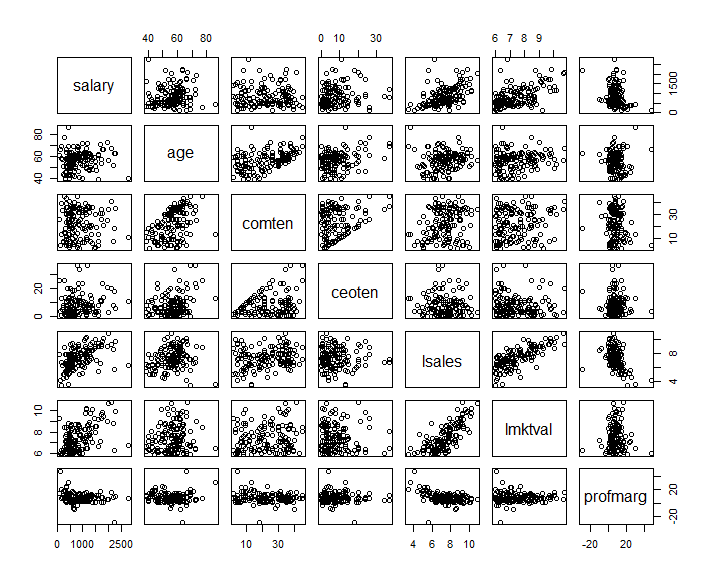
\includegraphics[width=.7\linewidth]{../Photo Of Result/B1_plotVriables.png}  
	\caption{Mối tương quan giữa các biến}
	\label{fig-b1:plot-vars}
\end{figure}

\begin{figure}[H]
	\centering
	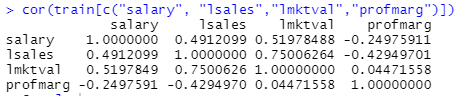
\includegraphics[scale = 0.6]{../Photo Of Result/B1_CorTable.PNG}  
	\caption{Mức độ tương quan giữa biến lsales và promarg Correlation}
	\label{fig-b1:corr-table}
\end{figure}

Xét bảng correlation giữa các biến độc lập với nhau và giữa các biến độc lập với biến phụ thuộc, ta thấy: Giữa hai biến $\textit{lmktval}$ và biến $\textit{lsales}$ có mối tương quan rất cao ($\approx$ 0.75). Tuy nhiên biến $\textit{lmktval}$ lại có mối tương quan cao hơn với biến phụ thuộc $\textit{salary}$. Mặt khác giữa biến $\textit{profmarg}$ và $\textit{lsales}$ cũng có mối tương quan cao ($\approx$ -0.42). Nên ta loại bỏ biến $\textit{lsales}$ khỏi danh sách các biến được xét. (2)

Từ (1) và (2) ta có mô hình với đầy đủ các biến cần lựa chọn như sau:
\begin{equation}\label{eq-b1:full-model}
	\begin{split}
		salary 	= \beta_0 + &\beta_1*age + \beta_2*college + \beta_3*grad + \beta_4*comten\\
		&+ \beta_5*ceoten + \beta_6*lmktval + \beta_7*profmarg
	\end{split}
\end{equation}


Thực hiện phân rã hai biến phân loại gồm $college$ và $grad$ trước khi thực hiện phương~pháp chọn biến \textbf{Stepwise} \textbf{tiến} với \textbf{tiêu chuẩn AIC}.

Để đánh giá chất lượng mô hình ta chia tâp dữ liệu thành hai phần, training và testing, với tỷ lệ $80:20$ sau đó tiến hành phương pháp chọn biến trên tập training.

\subsection*{Thực hiện chọn biến bằng phương pháp StepWise tiến và tiêu chuẩn AIC}

%\begin{figure}[H]
%	\centering
%	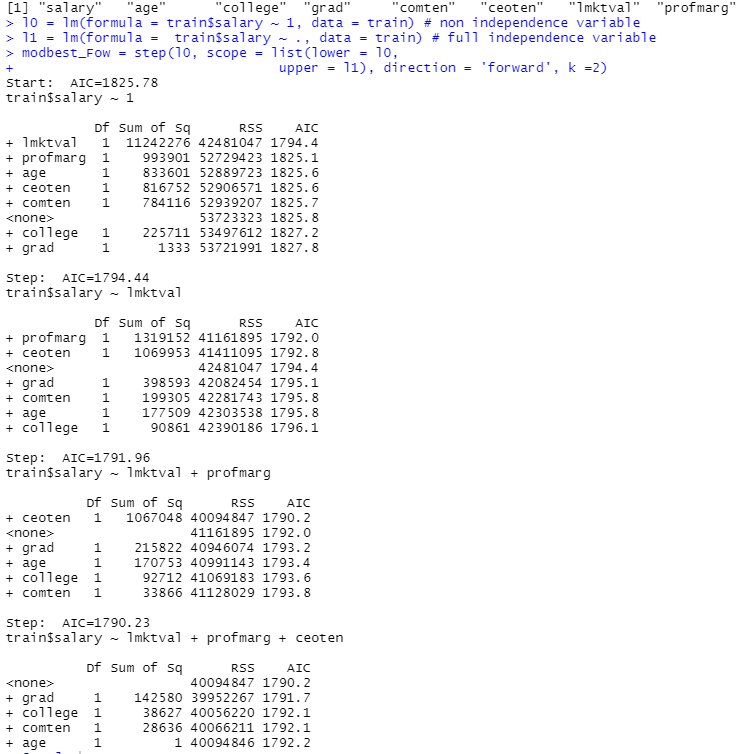
\includegraphics[scale = 0.52]{../Photo Of Result/B1_stepwiseForward.PNG}  
%	\caption{Kết quả chọn biến theo phương pháp StepWise tiến với tiêu chuẩn AIC}
%	\label{fig-b1:stepwise-forward}
%\end{figure}

Tổng quan tiêu chuẩn AIC thì mô hình tốt là mô hình có giá trị AIC nhỏ nhất. Ở mô hình 1, biến $\textit{lmktval}$ được chọn vào mô hình vì có AIC nhỏ nhất trong tất cả các kết~hợp với các biến còn lại. Tương tự AIC được tính cho mô hình thêm biến thứ 2, $\textit{ceoten}$, và biến thứ 3 là $\textit{ceoten}$ (hình \ref{ex1:model:1}).

\begin{figure}[H]
	\centering
	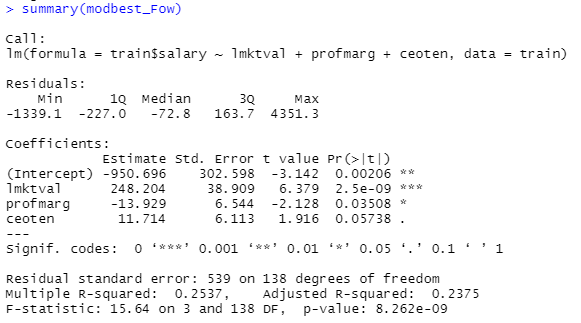
\includegraphics[width=.7\linewidth]{../Photo Of Result/B1_summary.PNG}  
	\caption{Kết quả hồi quy mô hình với các biến được chọn}
	\label{ex1:model:1}
\end{figure}

Với ba biến được chọn ở trên, mô hình \ref{eq-b1:full-model} trở thành mô hình mới:
\begin{equation}\label{1.2}
\textit{salary} = -950.6 + 248.2 * \textit{lmktval} - 13.9 *\textit{profmarg} + 11.7  *\textit{ceoten}
\end{equation}
Tuy nhiên ta nhận thấy biến $\textit{ceoten}$ có $\rho_{value} \ge \alpha$ (0.05738 $\ge$ 0.05) nên không có ý~nghĩa thống kê trong mô hình. Ta tiến hành bỏ biến $\textit{ceoten}$ và hồi quy mô hình với hai biến còn lại kết quả thu được từ phần mềm R như hình \ref{fig-b1:new-summary}:

\begin{figure}[H]
	\centering
	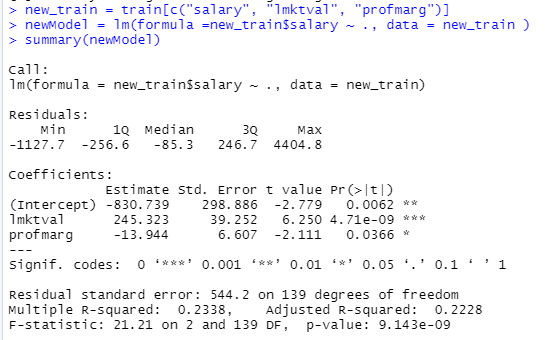
\includegraphics[width=.7\linewidth]{../Photo Of Result/B1_newsummary.PNG}  
	\caption{Kết quả hồi quy mô hình với hai biến còn lại}
	\label{fig-b1:new-summary}
\end{figure}

Mô hình thống kê mới:
\begin{equation}\label{1.3}
\textit{salary} = -830.7 + 245.3 *\textit{lmktval} -13.9 *\textit{profmarg}
\end{equation}

Trường hợp này hai biến còn lại có ý nghĩa thống kê. Tuy nhiên mô hình được tạo bởi hai biến này chỉ giải thích được 23$\%$ sự biến thiên của biến phụ thuộc (hình \ref{fig-b1:new-summary}). Nguyên nhân dẫn tới kết quả thấp là do số lượng data ít, các biến giải thích ít không tạo nên mô hình đặc trưng được.

\subsection*{Test trên tập test và nhận xét kết quả}

Thực hiện dự đoán trên tập dữ liệu test từ kết quả mô hình \ref{1.3} và dùng chỉ số đánh giá MSE (trung bình bình phương sai số) ta có:

\begin{figure}[H]
	\centering
	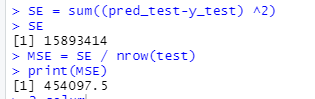
\includegraphics[width=.5\linewidth]{../Photo Of Result/B1_MSE.PNG}  
	\caption{Chỉ số đo lường kết quả MSE}
	\label{fig-b1:mse}
\end{figure}
